\section{Transient absorption spectroscopy}
\label{sec:TheoTransAbs} 

In the following section, the effect of transient absorption spectroscopy is explained. 

The above-mentioned method reveals information about the energetic structure of the material. With transient absorption spectroscopy, we introduce a second step of measurement by incorporating an adjustable time delay between two laser pulses. This adjustable time delay is realized in the setup as shown in (ref) with a length-adjustable beam path in the second beam path.
 
After the first pulse, we introduce a second laser pulse, which is weaker, with a controllable delay time denoted as $\tau$. This delayed pulse interacts with the matter in its excited state. The interaction of the delayed pulse with the material leads to three observable effects in the spectrum: \textit{Ground State bleaching} (GSB), \textit{transient absorption} (TA), and \textit{stimulated emission} (SE) schematically depicted in (fig). 
\begin{figure}[ht]
    \centering
    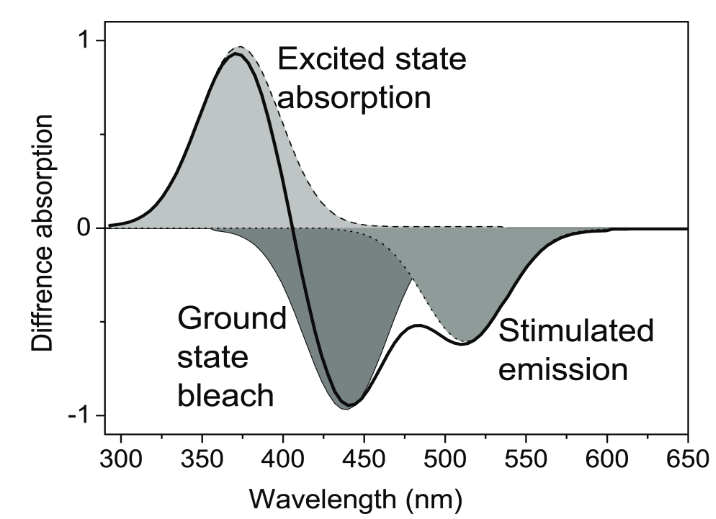
\includegraphics[width = 12cm]{Bilder/Grundlagen/GSBSETA.png}
    \caption{The three effects in transient absorption spectroscopy: Ground state bleaching, transient absorption and stimulated emission. The peak position between GSB and SE is called \textit{Stokes shift}. From \cite{5796fb6fae874c3fb73b57f57c942314}}
    \label{fig:GSBSETRA}
\end{figure}
Ground-state bleaching occurs because of the excitation process. The lowered ground-state density absorbs less light. This lowering in absorption is called \textit{ground state bleaching}. Transient absorption is the further excitation of an excited state with a second photon. 
Transient absorption spectroscopy gives insight into energy transfer and charge transfer dynamics of the material systems. For the effects mentioned effects to be visible, the intensity of the first LASER puls has to be 
sufficiently large.


